\documentclass[10pt,
               hyperref={bookmarks=false,
                         bookmarksopen=false,
                         colorlinks=true,
                         linkcolor=blue,
                         urlcolor=blue},
               xcolor={svgnames,table}]{beamer}

\usetheme[sectionpage=simple]{metropolis}
\usepackage{appendixnumberbeamer}

\usepackage{booktabs}
\usepackage[scale=2]{ccicons}
\usepackage{pgfplots}
\usepgfplotslibrary{dateplot}
\usepackage[export]{adjustbox}
\usepackage{hyperref}
\usepackage[T1]{fontenc}
\usepackage[svgnames]{xcolor}
\usepackage{xspace}
\usepackage{changepage}
\usepackage{epigraph}

\newcommand{\themename}{\textbf{\textsc{metropolis}}\xspace}
\setbeamercolor{background canvas}{bg=white}
\setbeamercolor{title}{fg=blue}
\setbeamercolor{date}{fg=blue}
\setbeamercolor{frametitle}{bg=yellow, fg=blue}
\setbeamertemplate{footline}[page number]
\setbeamerfont{section title}{size=\Huge, series=\bfseries}
\setbeamertemplate{itemize item}[circle]
\setbeamercolor{itemize item}{fg=blue}

\newcommand{\sectionframe}[1]{
  \begin{frame}{\thetitle}
    \section{#1}
  \end{frame}
}

\newcommand\blfootnote[1]{%
  \begingroup
  \renewcommand\thefootnote{}\footnote{#1}%
  \addtocounter{footnote}{-1}%
  \endgroup
}
% tight itemized list
\newenvironment{tightitemize}{%
\begin{itemize}
  \setlength{\itemsep}{1pt}%
  \setlength{\parskip}{0pt}%
  \setlength{\parsep}{0pt}%
}{\end{itemize}}

% paperref{title}{authors}{journal}{doi}
\newcommand\paperref[4]{%
  {\it #1, }{ #2,}{ #3}
}

% -----------------------------------------------------------------------------
\newcommand{\thetitle}{GENCODE at UCSC 2018}
\title{\vspace{2cm}\thetitle}
\date{June 21-22, 2018}
\author[markd]{
    Mark Diekhans \href{mailto:markd@ucsc.edu}{\textless markd@ucsc.edu\textgreater} \\
    Joel Armstrong \href{mailto:jcarmstr@ucsc.edu}{\textless jcarmstr@ucsc.edu\textgreater} \\
    Benedict Paten \href{mailto:bpaten@ucsc.edu}{\textless bpaten@ucsc.edu\textgreater} \\
    Adam Novak (graph genomes) \\
    Mark Akeson, Miten Jain (nanopore) \\
    Ian Fiddes, Stefanie Nachtweide (emeritus) \\
}

\titlegraphic{\hfill
\includegraphics[height=1.5cm]{images/Genomics_Institute_Logo_Pathed_Text.pdf}}
\begin{document}

\maketitle

\begin{frame}{Outline}
  \setbeamertemplate{section in toc}[sections numbered]
  \tableofcontents[hideallsubsections]
\end{frame}

% -----------------------------------------------------------------------------
\sectionframe{Introduction}

\begin{frame}{The three As of comparative genomics}
  \begin{center}
    \begin{adjustwidth}{-0.8em}{-0.8em}
      \only<1>{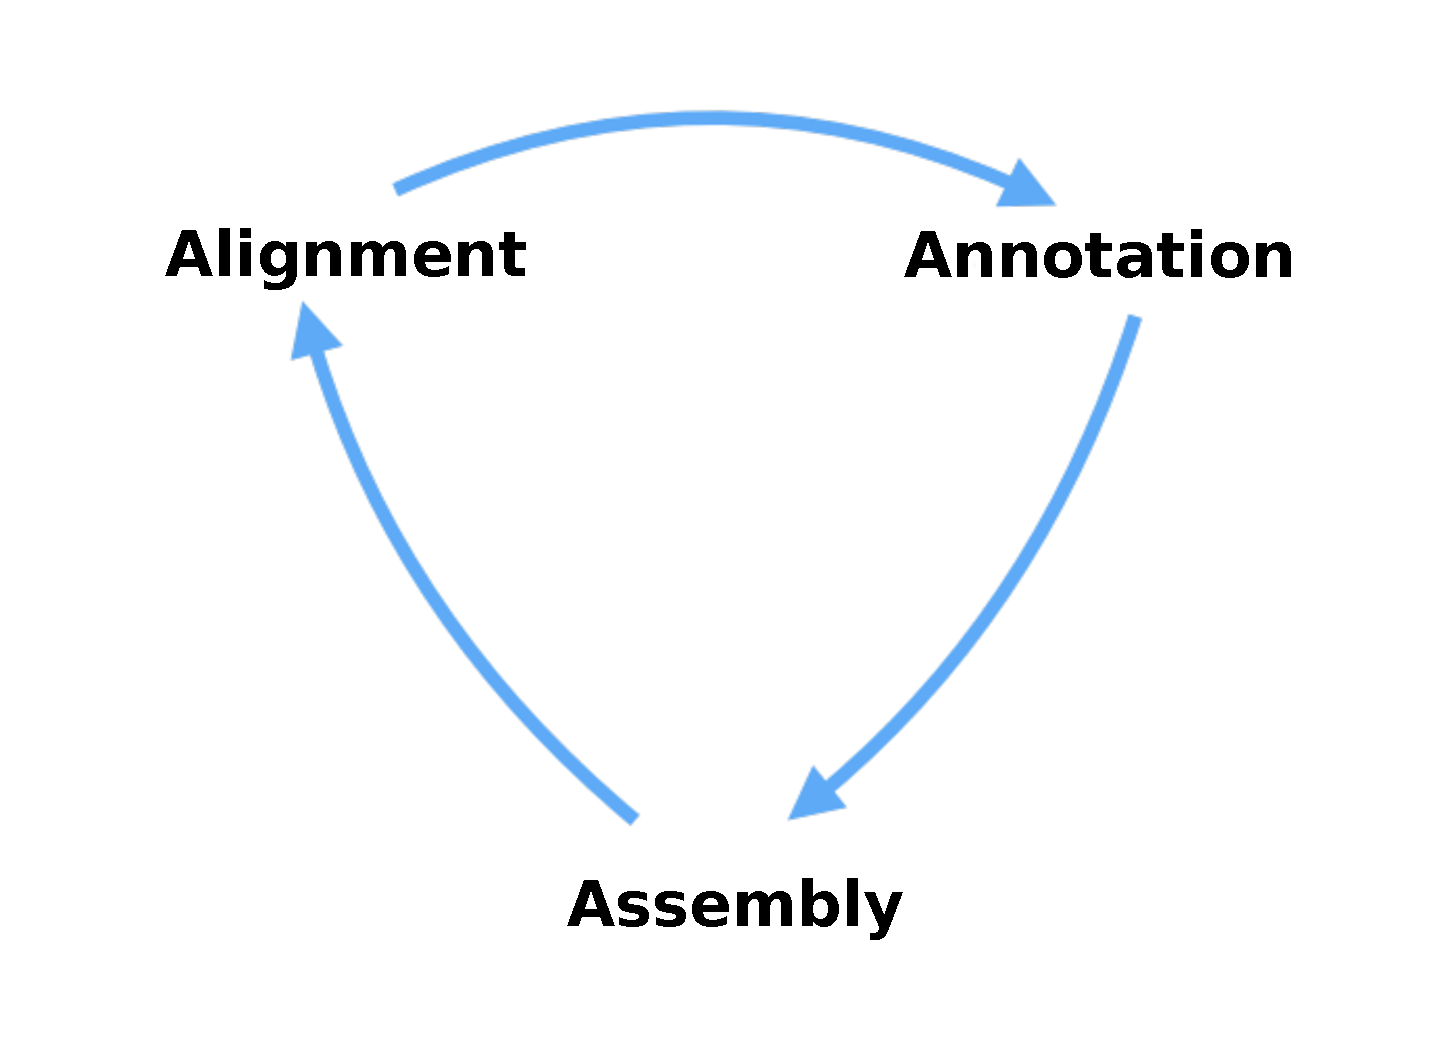
\includegraphics[scale=0.45]{images/three-As.pdf}}
      \only<2>{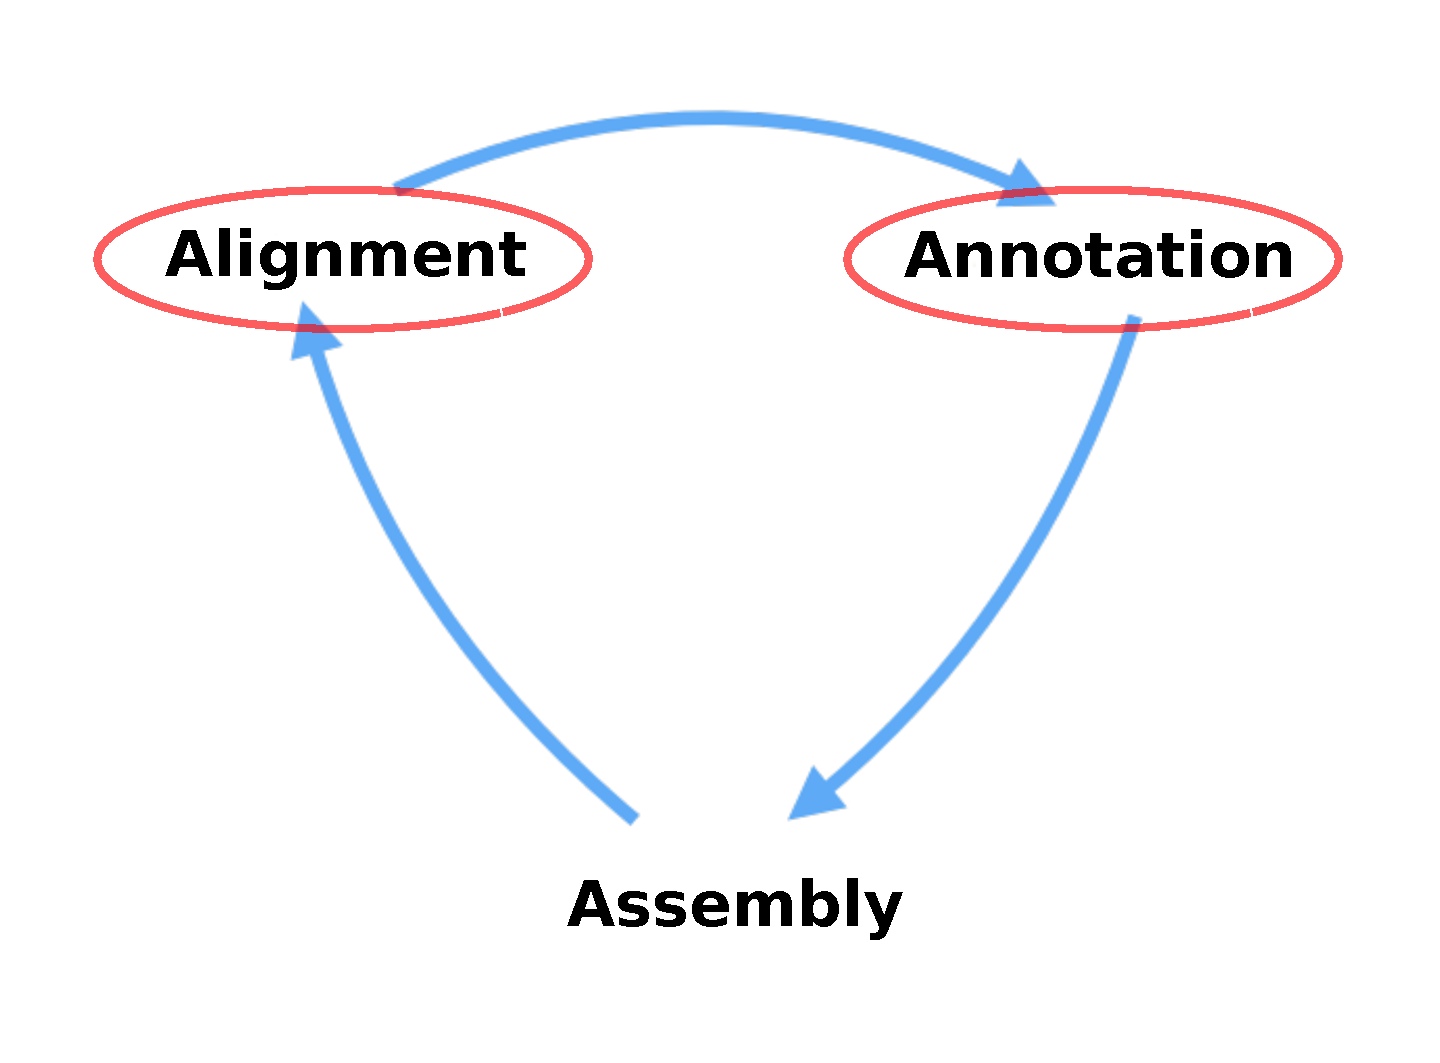
\includegraphics[scale=0.45]{images/our-two-As.pdf}}
    \end{adjustwidth}
  \end{center}
\end{frame}

\begin{frame}{Comparative genomics as an annotation tool}
  \begin{columns}
    \begin{column}{0.80\textwidth}
      \begin{tightitemize}
      \item \paperref{Long-read sequence assembly of the gorilla genome}
        {Gordon et al.}{Science Apr 2016}{10.1126/science.aae0344}
      \item \paperref{High-resolution comparative analysis of great ape genomes}
        {Kronenberg, et al.}{Science June 2018}{10.1126/science.aar6343}
      \item \paperref{Repeat associated mechanisms of genome evolution and function revealed by the Mus caroli and Mus pahari genomes}
        {Tybert, et al.}{Genome Res. Apr 2018}{10.1101/gr.234096.117}
      \item \paperref{Mouse strain genomes project, 16 laboratory and wild-derived strains}
        {Lilue, et al.}{accepted}{}
      \item \paperref{Evaluating recovery potential of the northern white rhinoceros from cryopreserved somatic cells}
        {Tunstal, et al.}{Genome Res. 2018}{10.1101/gr.227603.117}
      \end{tightitemize}
    \end{column}
    \begin{column}{0.20\textwidth}
      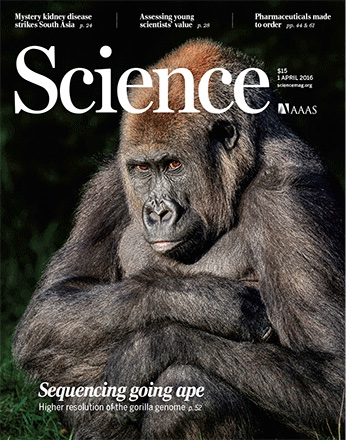
\includegraphics[scale=0.2]{images/science-gorilla.jpg}
      \vspace{4em}
      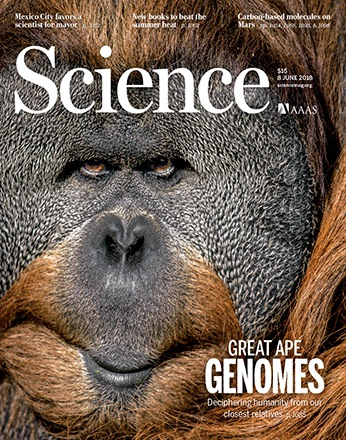
\includegraphics[scale=0.2]{images/science-ape.jpg}
    \end{column}
  \end{columns}
\end{frame}

% -----------------------------------------------------------------------------
\sectionframe{Comparative genomics alignment}

\begin{frame}{Cactus}
  \begin{columns}
    \begin{column}{0.5\textwidth}
      \begin{itemize}
          \item Cactus is a non-reference-biased, whole-genome multiple-alignment tool
          \item Most genome multiple alignments are reference-biased: for any two non-reference genomes, any homologies between sequence not present in the reference are not aligned
          \item Reference-free alignments are harder to generate, but valuable for many comparative genomics applications
      \end{itemize}
    \end{column}
    \begin{column}{0.5\textwidth}
      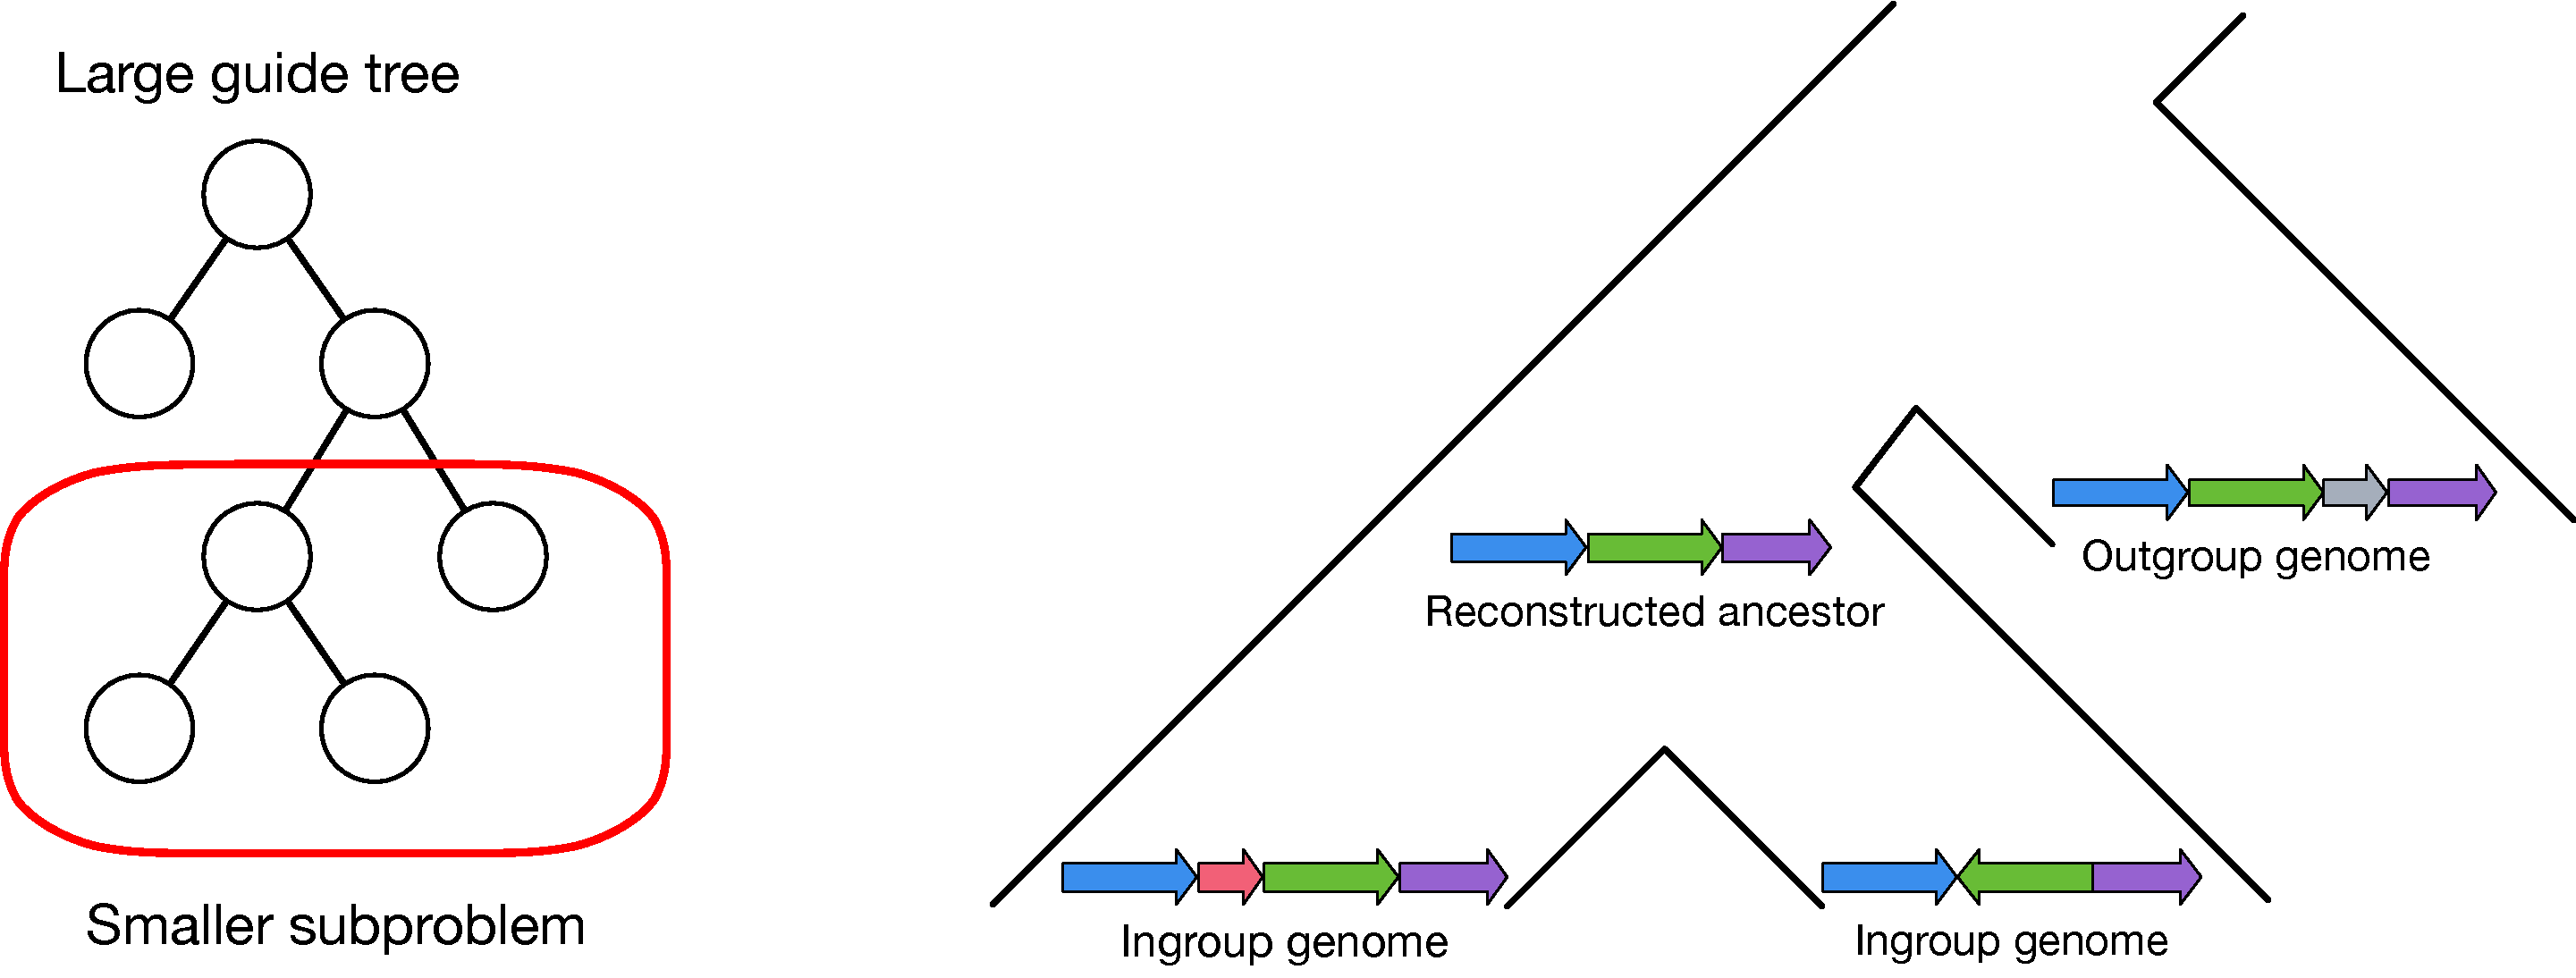
\includegraphics[width=\columnwidth]{images/progressive-alignment-and-reconstruction-minus-labels.pdf} \\
      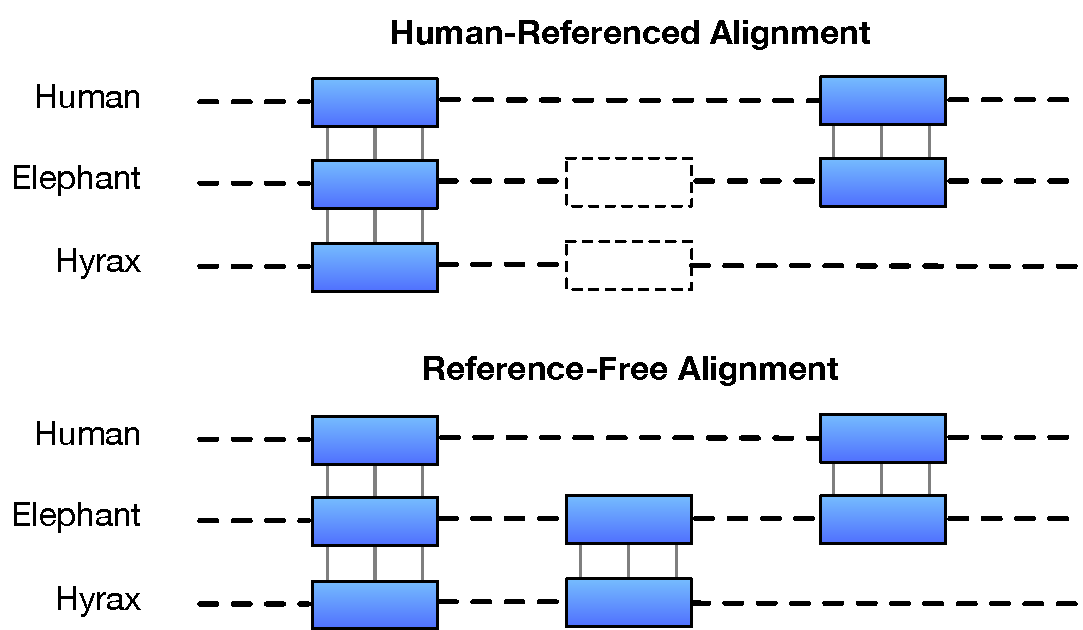
\includegraphics[width=\columnwidth]{images/reference-free-diagram.pdf}
    \end{column}
  \end{columns}
\end{frame}

\begin{frame}{Cactus enables very-large-scale comparative genomics}
    \begin{itemize}
        \item Sequencing projects are becoming larger and larger as the cost of sequencing continues to fall
        \item Several large projects are aiming to sequence hundreds to thousands of genomes in the coming years
        \item Aligning at this scale is very difficult
          \begin{tightitemize}
          \item Cactus was explicitly designed for these very large alignments
          \end{tightitemize}
        \item Thanks to long-read technology, there are already many more gold-standard assemblies that are worthy of being studied in detail, making reference-free alignments more important
        \item \emph{The dream}: a single, frequently-updated public resource which relates thousands of vertebrate genomes to one another and allow information/annotation transfer across species, viewable from any genome
          \begin{tightitemize}
            \item As a first draft, we plan to create a 600+-way pan-tetrapod alignment combining two large sequencing \& analysis projects we are currently working on
        \end{tightitemize}
    \end{itemize}
\end{frame}

\begin{frame}{Bird 10K}
    \begin{columns}
        \begin{column}{0.5\textwidth}
            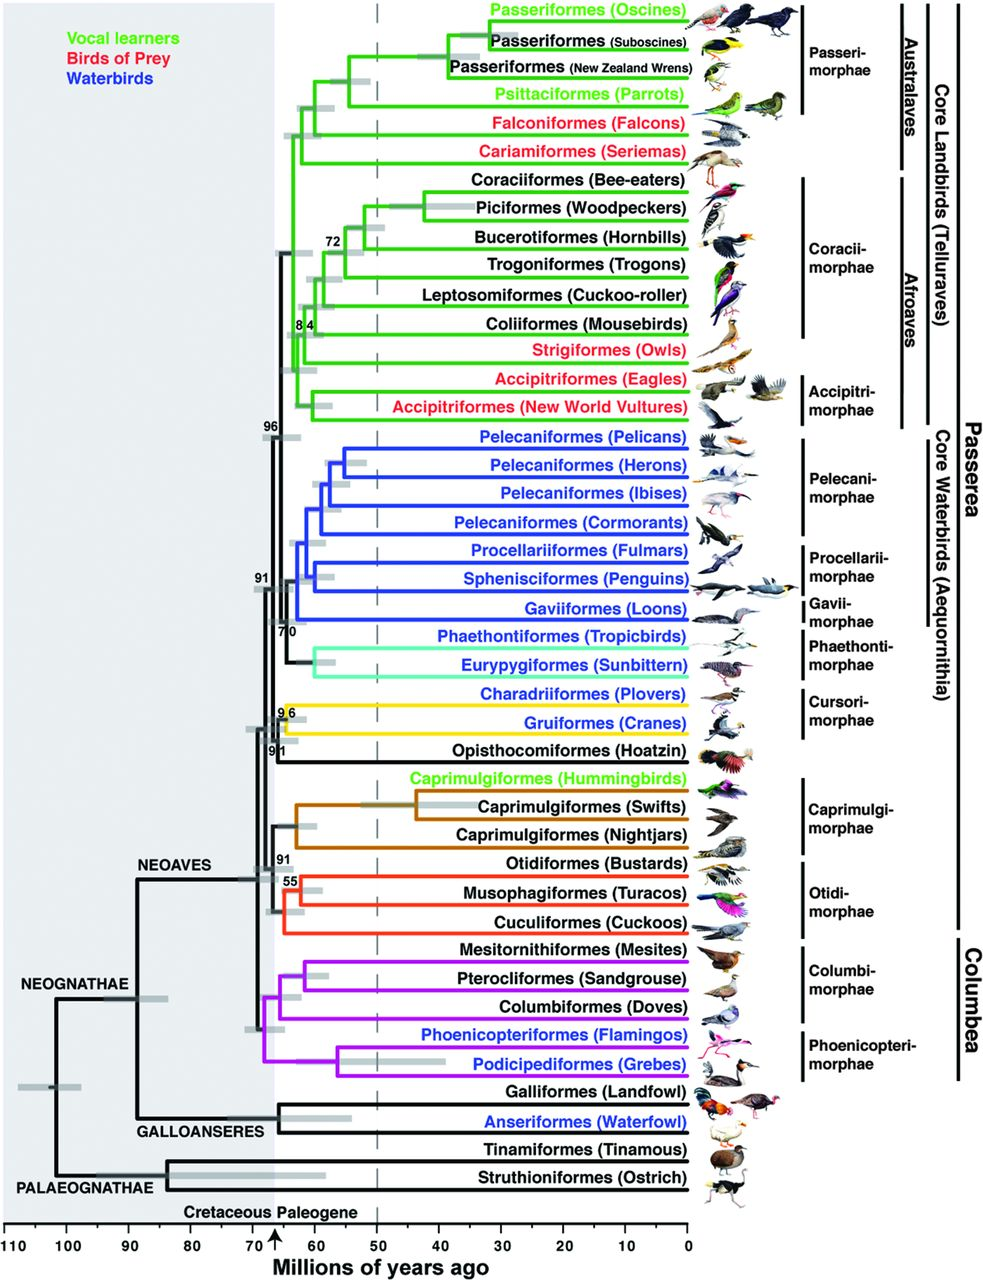
\includegraphics[width=\columnwidth]{images/B10K_tree.jpg}
        \end{column}
        \begin{column}{0.5\textwidth}
            \begin{itemize}
                \item Ambitious sequencing project in multiple years-long phases: \begin{itemize}
                    \item Phase 1: sequence 48 birds (one species from every order)
                    \item \textbf{\textcolor{DarkGreen}{Phase 2: sequence 300 birds (one species from every family)}}
                    \item Phases 3 and 4: all the rest! (\char`~9600)
                \end{itemize}
                \item How to enable analysis of this massive dataset without reference bias? Cactus!
                \item Large analysis project with many goals, but primarily to gain more insight about the species tree of birds
            \end{itemize}
        \end{column}
    \end{columns}
\end{frame}

\begin{frame}{200 Mammals}
  \begin{columns}
    \begin{column}{0.5\textwidth}
      \begin{itemize}
          \item Extending earlier 29 Mammals project: from 29 mammals spanning 4.5 subs/site to 252 mammals with \char`~15 subs/site
          \item Aligning using Cactus
          \item Generating 1bp-resolution constrained elements annotations (on human, but also on all other mammals!)
          \item Generating gene sets for all 252 assemblies using CAT
      \end{itemize}
    \end{column}
    \begin{column}{0.5\textwidth}
      \adjincludegraphics[trim={{0.2\width} 0 {0.2\width} 0},clip,width=\columnwidth]{images/200_Mammal_Tree.pdf}
    \end{column}
  \end{columns}
\end{frame}

% -----------------------------------------------------------------------------
\sectionframe{Comparative genomics annotation}

\begin{frame}{Comparative Annotation Toolkit (CAT)}
  \begin{itemize}
  \item Comparative annotation combining multiple sources of evidence
    \begin{tightitemize}
    \item Start with high-quality gene annotations on related species (GENCODE or Ensembl)
    \item Build cactus genomic alignments
    \item Project annotations through alignments to target genome
    \item Combine mappings with RNA-Seq and Iso-Seq evidence using AUGUSTUS gene finder (Mario Stanke)
    \item Create consensus gene set 
    \end{tightitemize}
  \item Developed by Ian Fiddes
  \item Ongoing maintenance 
  \item Work with Ensembl gene build group to incorporate useful methodologies
  \end{itemize}
\blfootnote{Comparative Annotation Toolkit (CAT) - simultaneous clade and personal genome annotation, Fiddes, et al., accepted; pre-print DOI:10.1101/231118}
\end{frame}

\begin{frame}{CAT pipeline}
  \begin{center}
    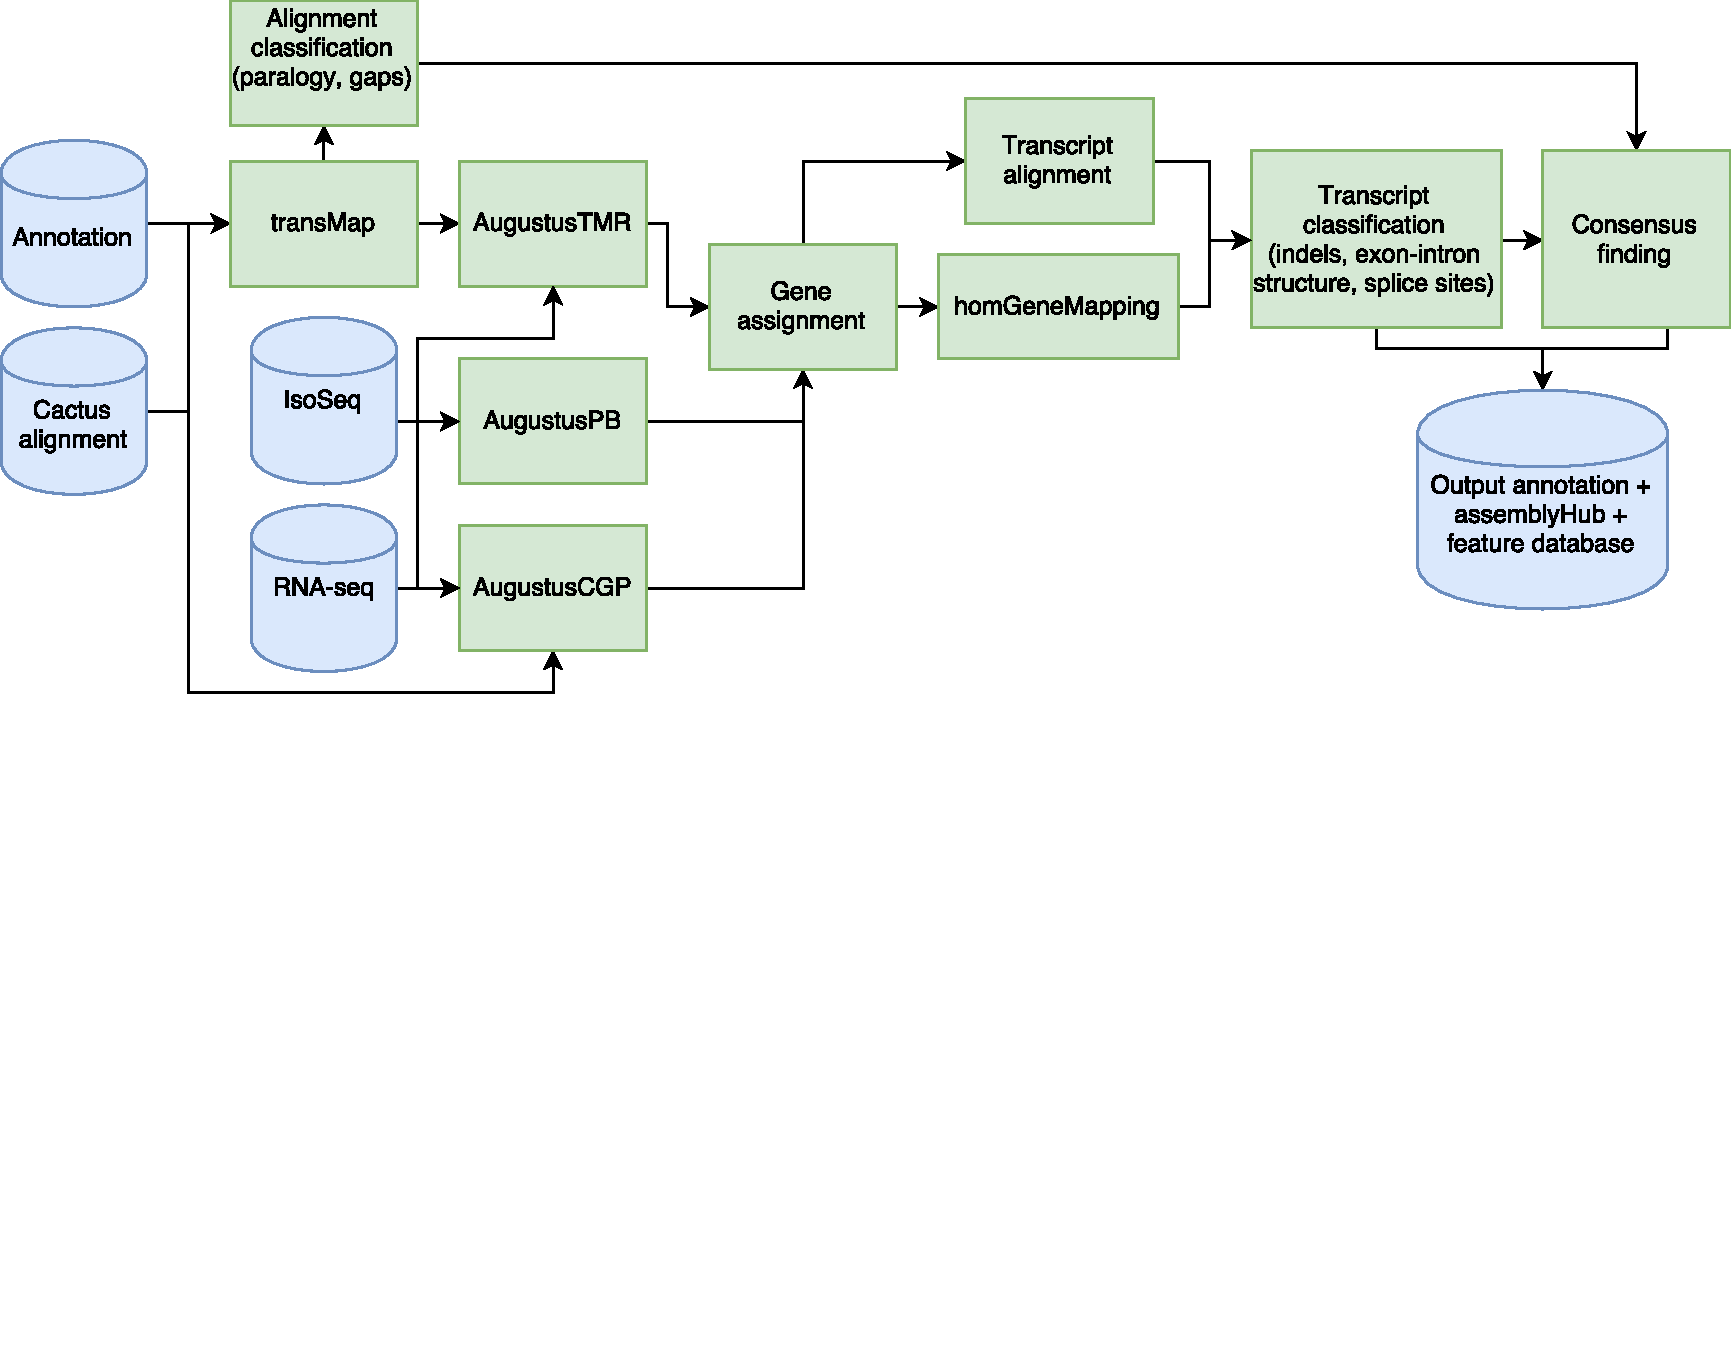
\includegraphics[scale=0.38]{images/CAT_pipeline.pdf}
  \end{center}
\end{frame}

% -----------------------------------------------------------------------------
\begin{frame}{\thetitle}
  \section{Graph genomes}
  {\large
  ``The biggest problem with graph genomes is people don't realize they need them.'' \\
  -- \textit{Deanna Church}}
\end{frame}

\begin{frame}{Graph genomes goals}
  \begin{itemize}
  \item Address reference-bias in genome-based analysis
  \item Consistent representation of human variation with at least 1\% penetrance
  \item Stable addressing as new variation is added
  \item Bring newer data to users stuck on older linear reference genome releases
  \item Support annotation of human variation (GENCODE pilot project)
  \end{itemize}
\end{frame}

\begin{frame}{Graph genomes basics}
  \begin{center}
    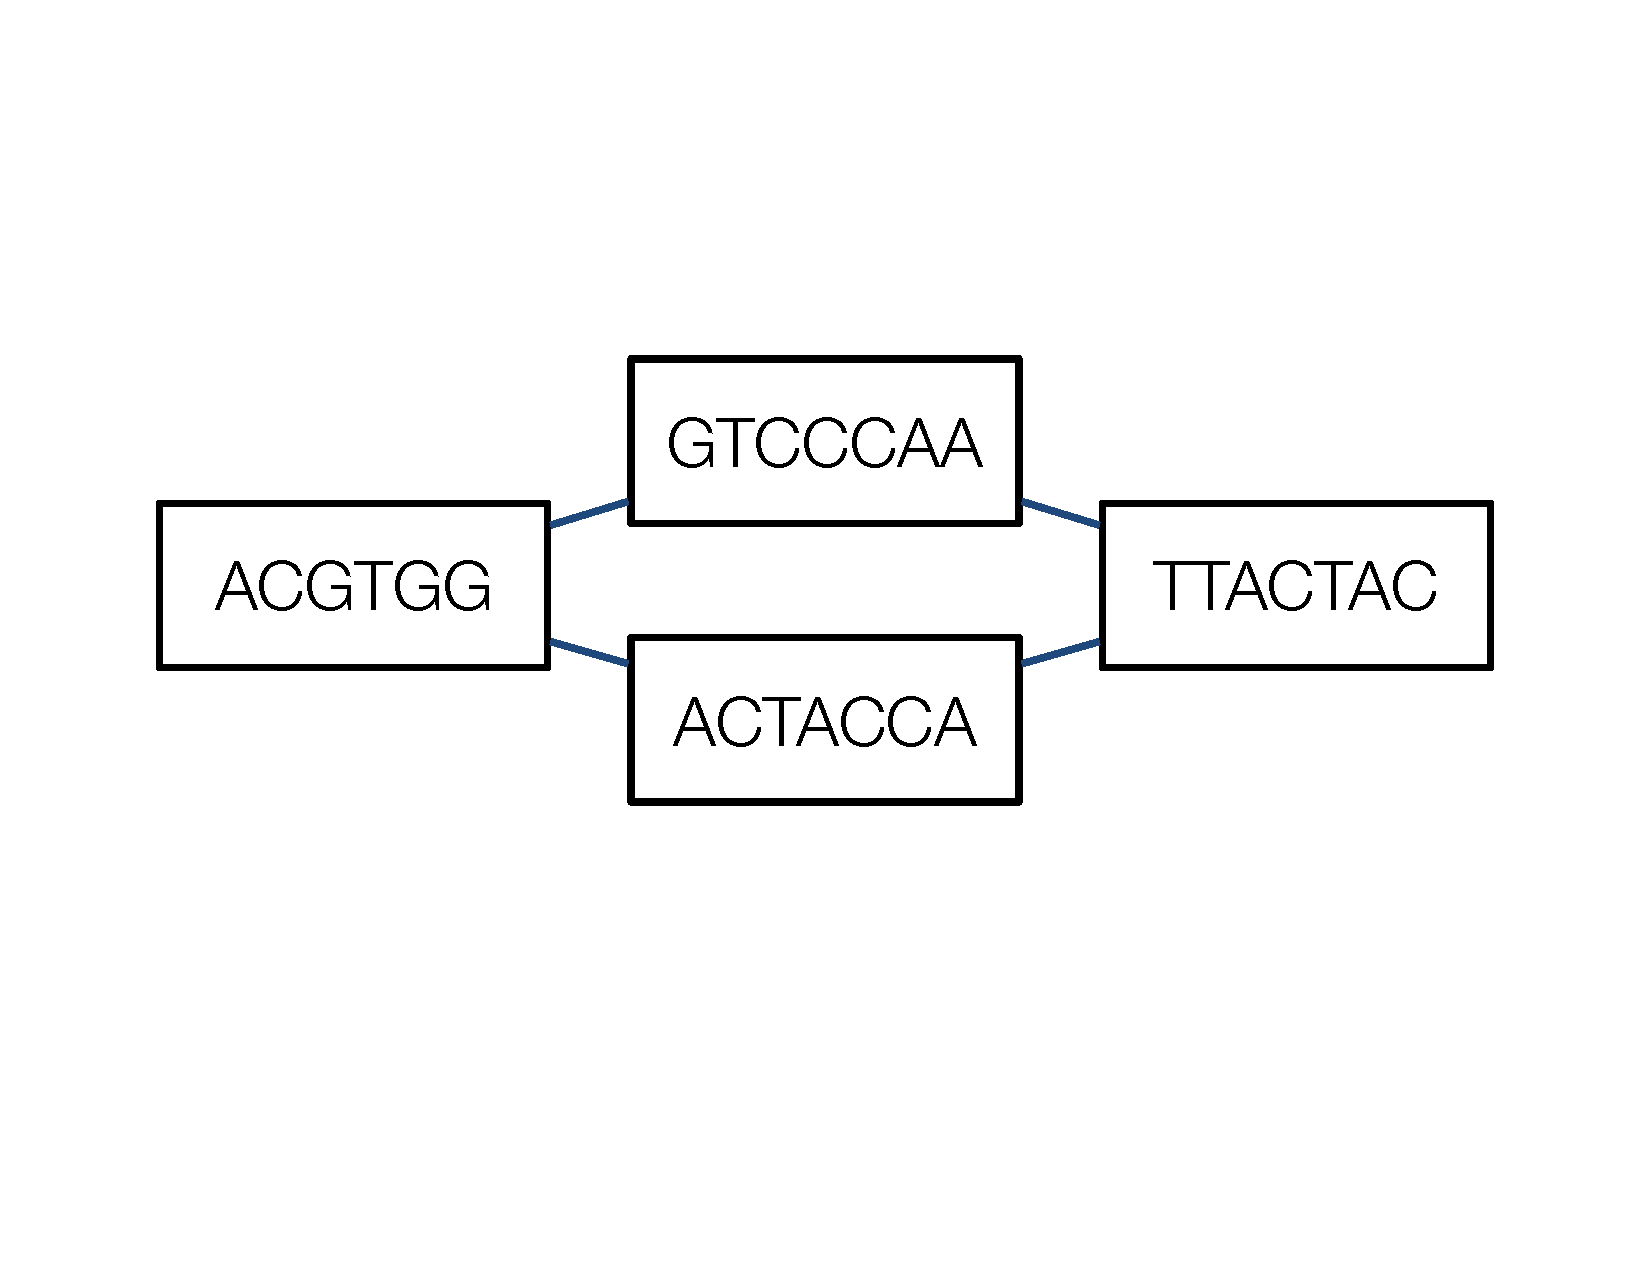
\includegraphics[scale=0.30]{images/graph-genome-alt.pdf} \\
    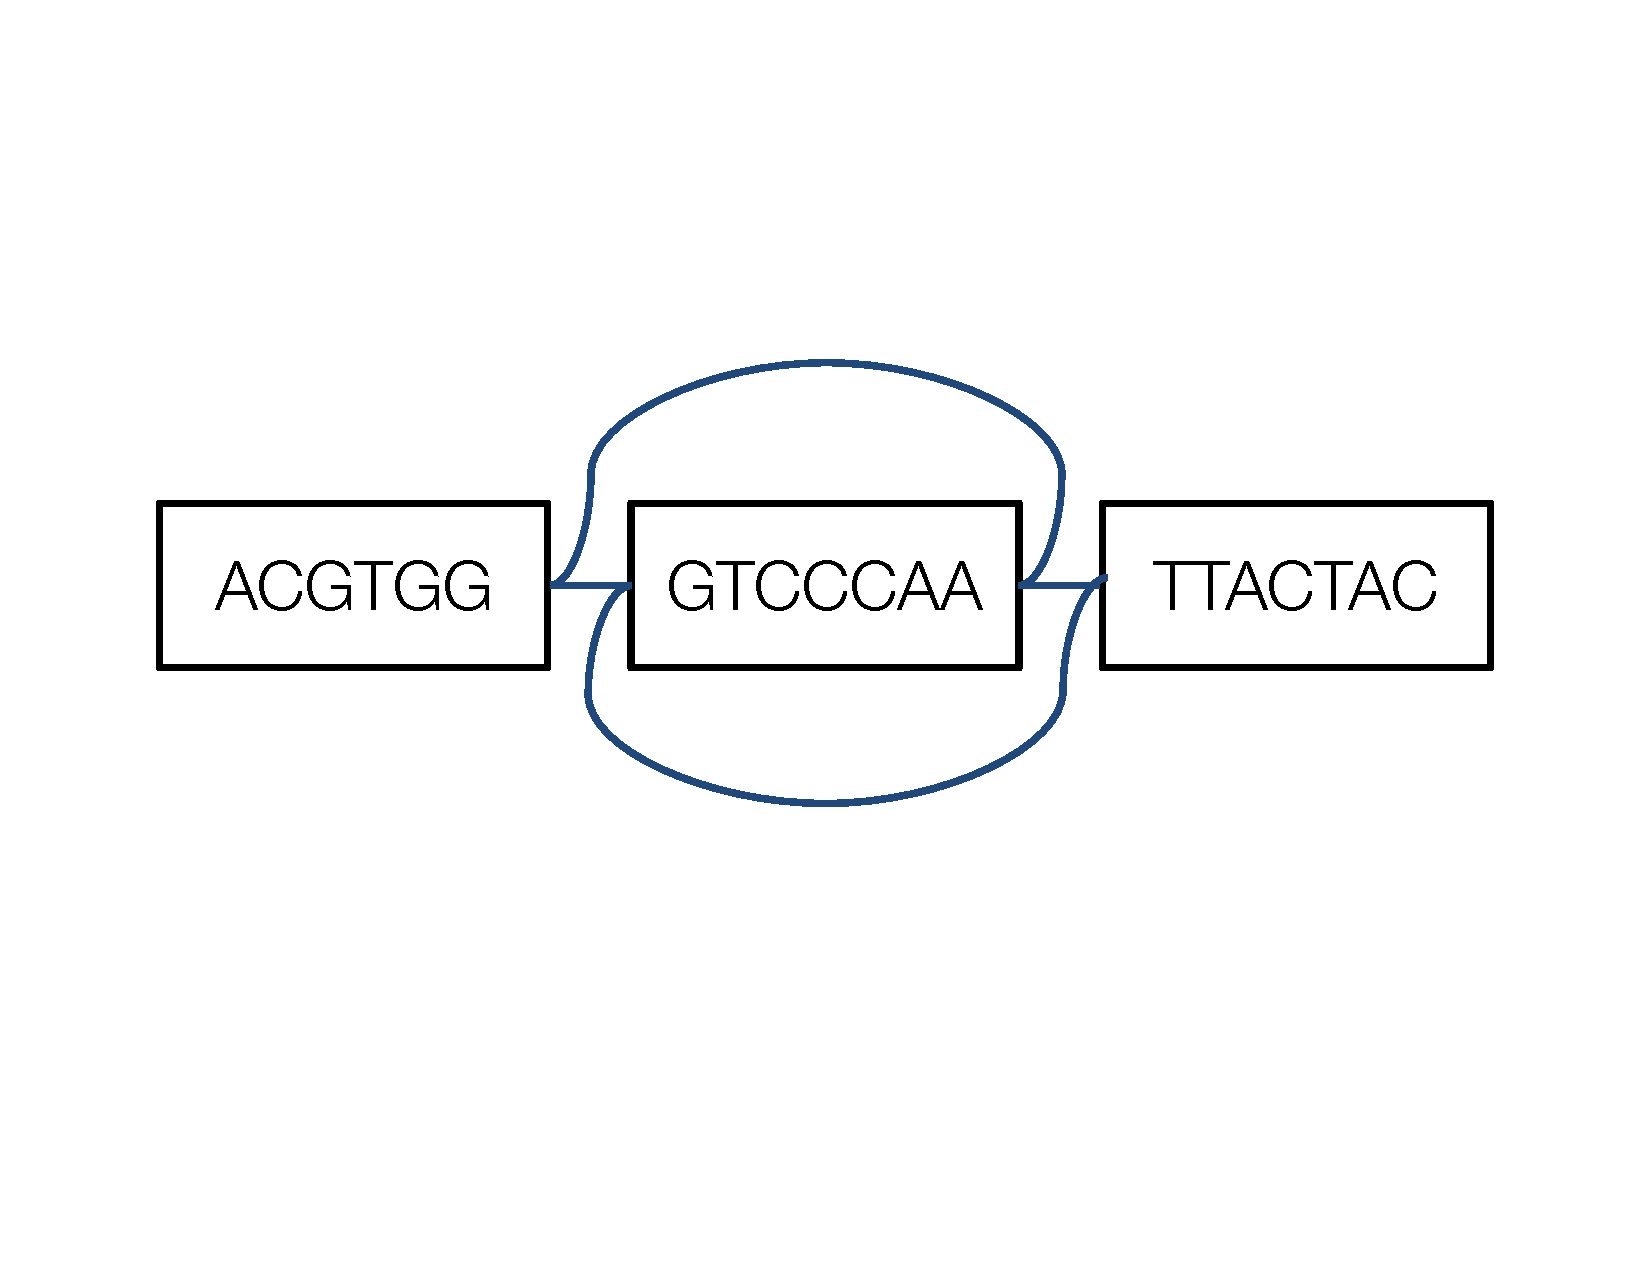
\includegraphics[scale=0.30]{images/graph-genome-inversion.pdf}
  \end{center}
  \begin{itemize}
  \item Set of sequences (nodes)
  \item Joins (edges) connect sides of sequences.
  \end{itemize}
\end{frame}

\begin{frame}{Graph genome representation complex variation (MHC)}
  \begin{center}
    \only<1>{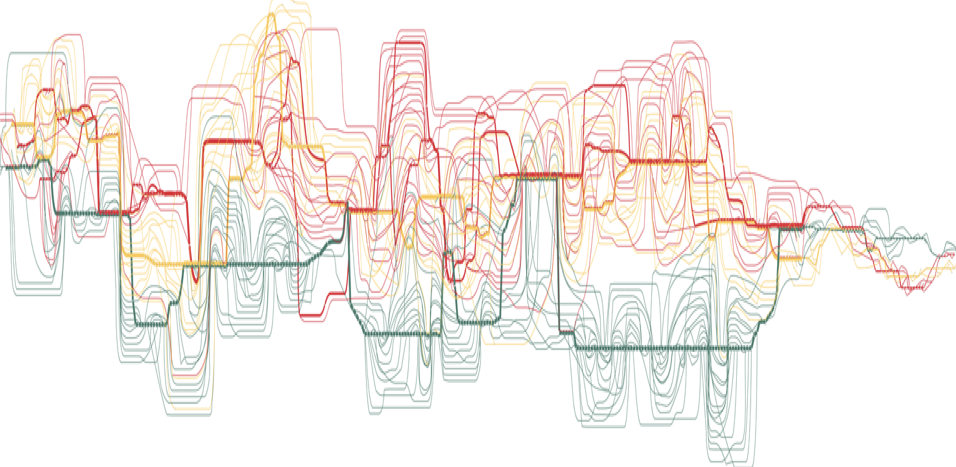
\includegraphics[scale=0.32]{images/graph-genome-mhc.png}}
    \only<2>{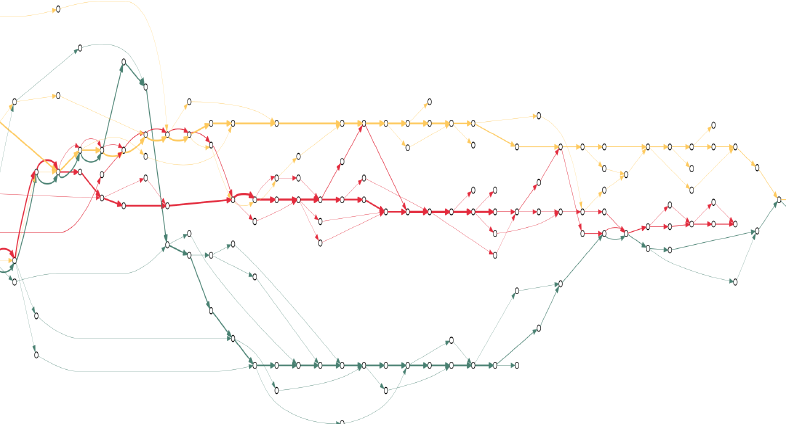
\includegraphics[scale=0.40]{images/graph-genome-local-structure.png}}
    \end{center}
  \blfootnote{The major histocompatibility complex - Kiran Garimella \& Gil McVean}
\end{frame}

\begin{frame}{Haplotypes are paths through a graph genome}
  \begin{center}
    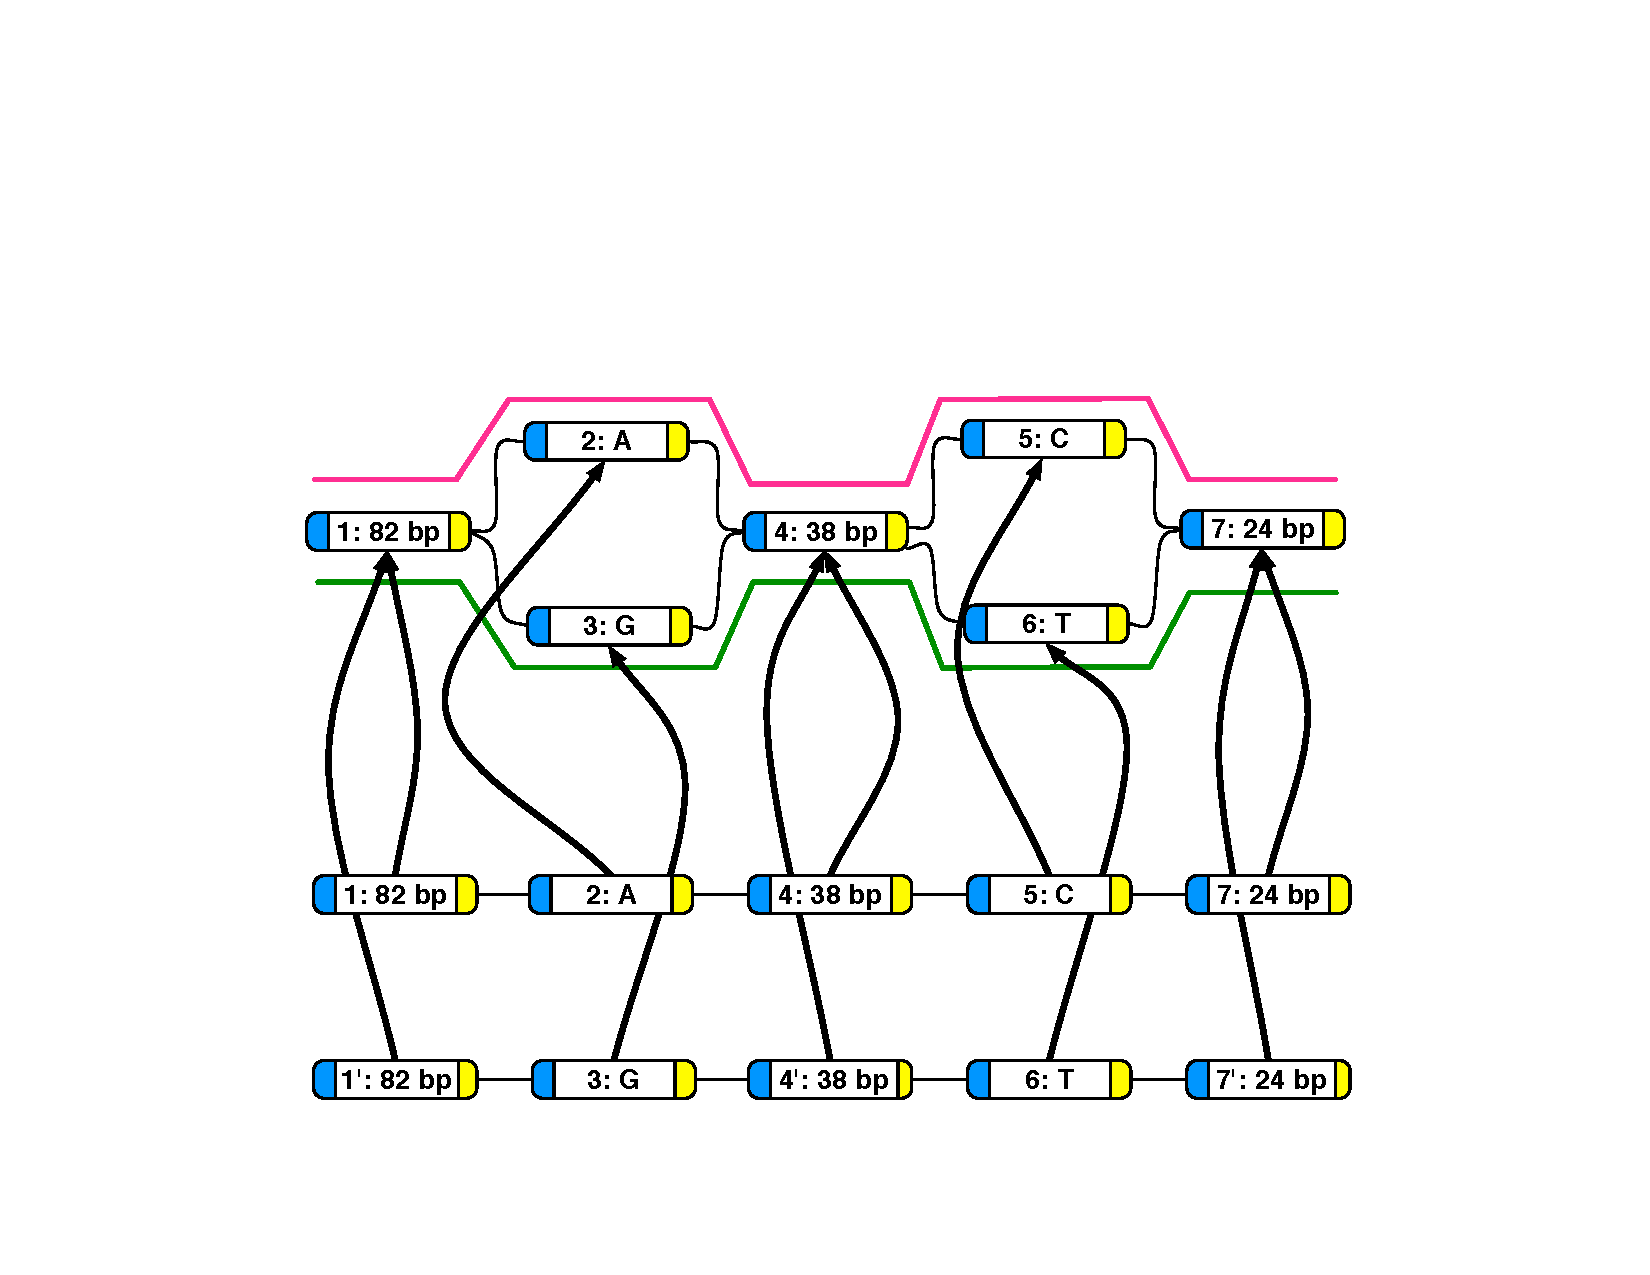
\includegraphics[scale=0.50]{images/graph-genome-haplotypes.pdf}
  \end{center}
\end{frame}

\begin{frame}{Annotating graph genomes}
  \begin{center}
    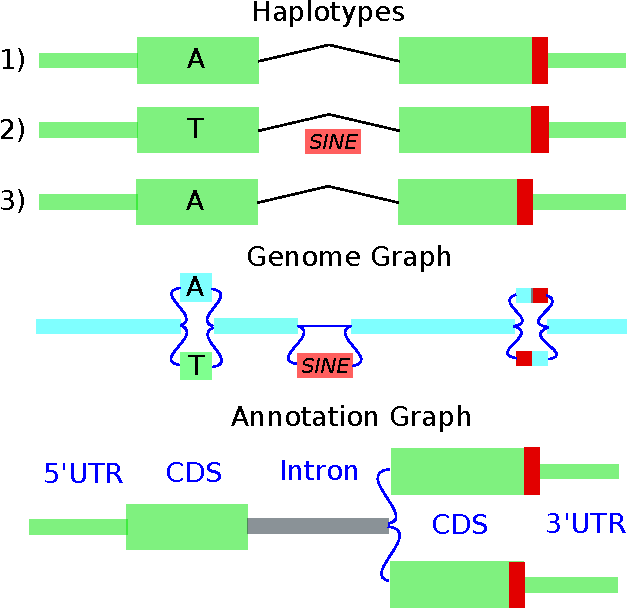
\includegraphics[scale=0.65]{images/graph-annotation.pdf}
  \end{center}
\end{frame}

% -----------------------------------------------------------------------------
\sectionframe{Transcript support}
\begin{frame}{Transcript support goals}
  \begin{itemize}
  \item Evaluate support of GENCODE annotations from current data
    \begin{tightitemize}
    \item Assist with annotations
    \item Guide users
    \end{tightitemize}
  \item Full-length support (TSL)
    \begin{tightitemize}
    \item GenBank \& dbEST 
    \item IsoSeq \& nanopore - the next step
    \end{tightitemize}
  \item Intron support (RSL)
    \begin{tightitemize}
    \item SRA/ENA open and controlled access RNA-Seq
    \end{tightitemize}
  \end{itemize}
\end{frame}

\begin{frame}{RNA-Seq intron support approaches}
  \begin{itemize}
  \item Large SRA cloud run
    \begin{tightitemize}
    \item Delayed by technology on free cloud resources
    \end{tightitemize}
  \item CZI SRA alignments
    \begin{tightitemize}
    \item 22k human \& 48k mouse experiments
    \item Random selection; many are small sets
    \item Approaching satiation, however many known introns missing
    \end{tightitemize}
  \item EBI Gene Expression Team collaboration
    \begin{tightitemize}
    \item Create an ongoing resource
    \end{tightitemize}
  \end{itemize}
\end{frame}

\begin{frame}<presentation:0>{CZI set experiment saturation for annotated introns}
  \begin{columns}
    \begin{column}{0.5\textwidth}
      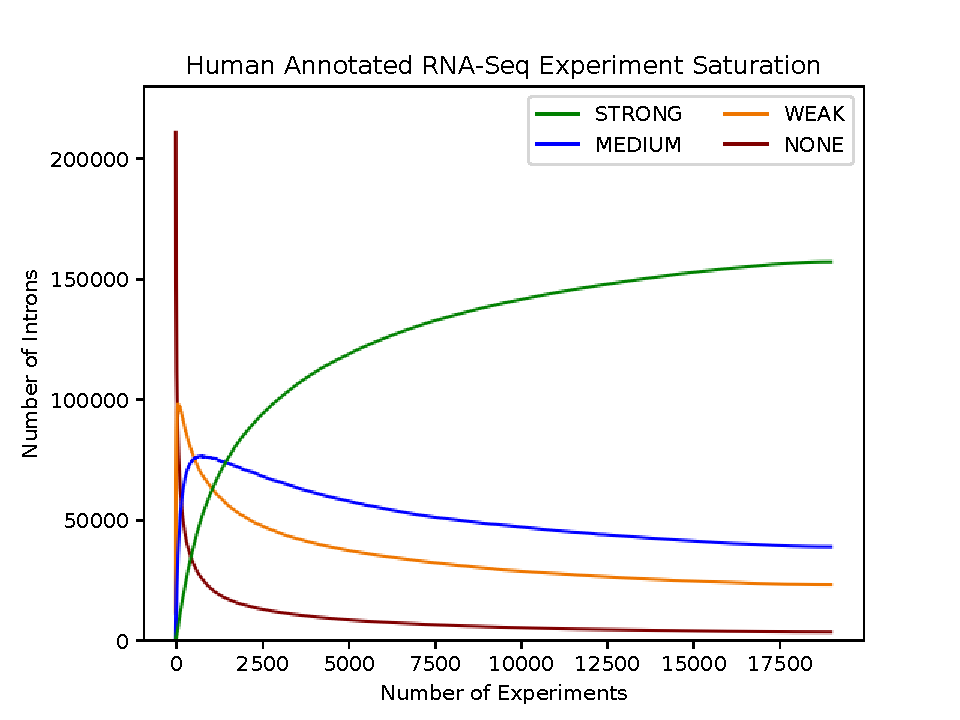
\includegraphics[scale=0.37]{images/hs_saturation_annot.pdf}
    \end{column}
    \begin{column}{0.5\textwidth}
      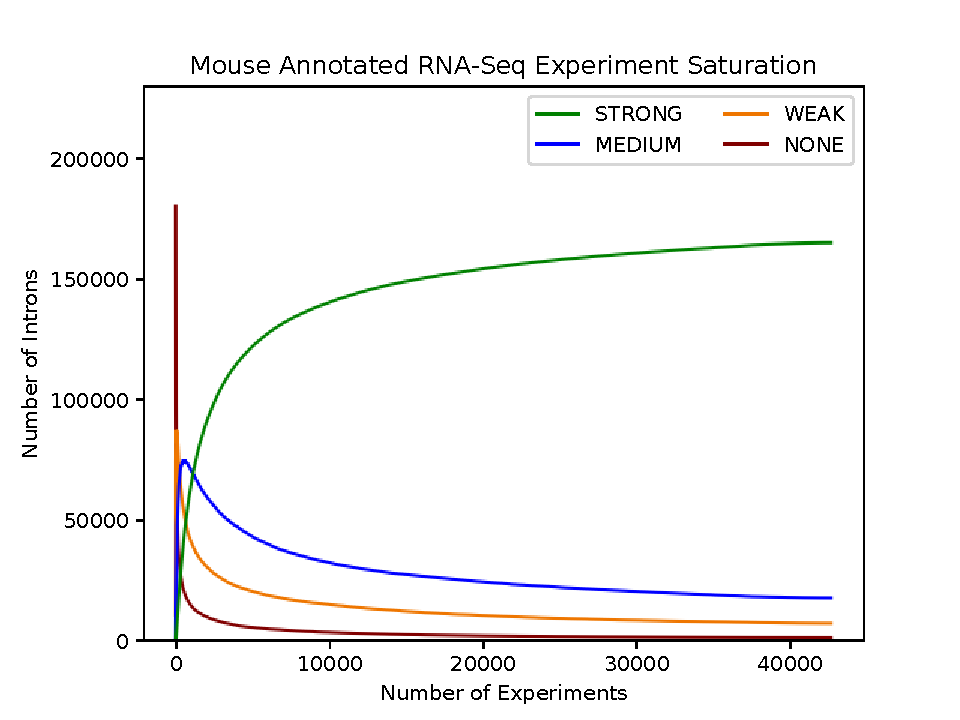
\includegraphics[scale=0.37]{images/mm_saturation_annot.pdf}
    \end{column}
  \end{columns}
\end{frame}

\begin{frame}{Expression Atlas collaboration}
  \begin{itemize}
  \item Expression Atlas pipeline currently maps with TopHat2 and estimates expression
    \begin{tightitemize}
    \item Process incoming RNA-Seq experiments; including controlled access
    \item Doesn't save splice junction calls
    \end{tightitemize}
  \item Redoing pipeline, most likely with {\em HISAT2}
  \item UCSC developed at intron caller that is independent of aligner
    \begin{tightitemize}
    \item \url{https://github.com/diekhans/intronProspector}
    \end{tightitemize}
  \item Provides data for all Ensembl assemblies, not just GENCODE
  \item UCSC will assist in initial recompute mouse using Azure cloud
  \end{itemize}
\end{frame}

\begin{frame}{Expression Atlas integration}
  \begin{center}
    Splice junction calling external to Expression Atlas
    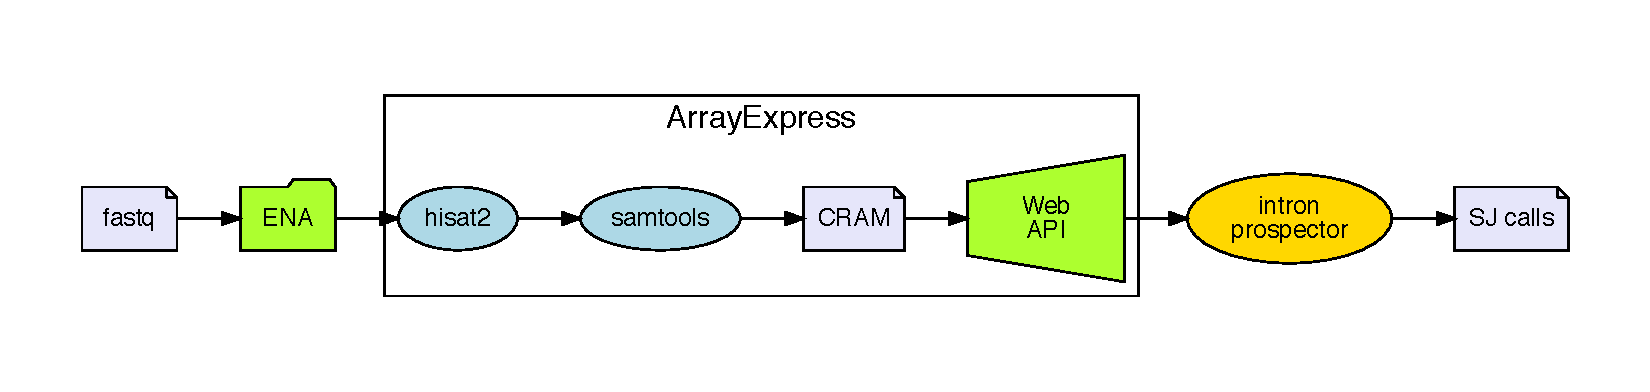
\includegraphics[scale=0.42]{images/calling_external.pdf}

    Splice junction calling in Expression Atlas RNA-Seq pipeline.
    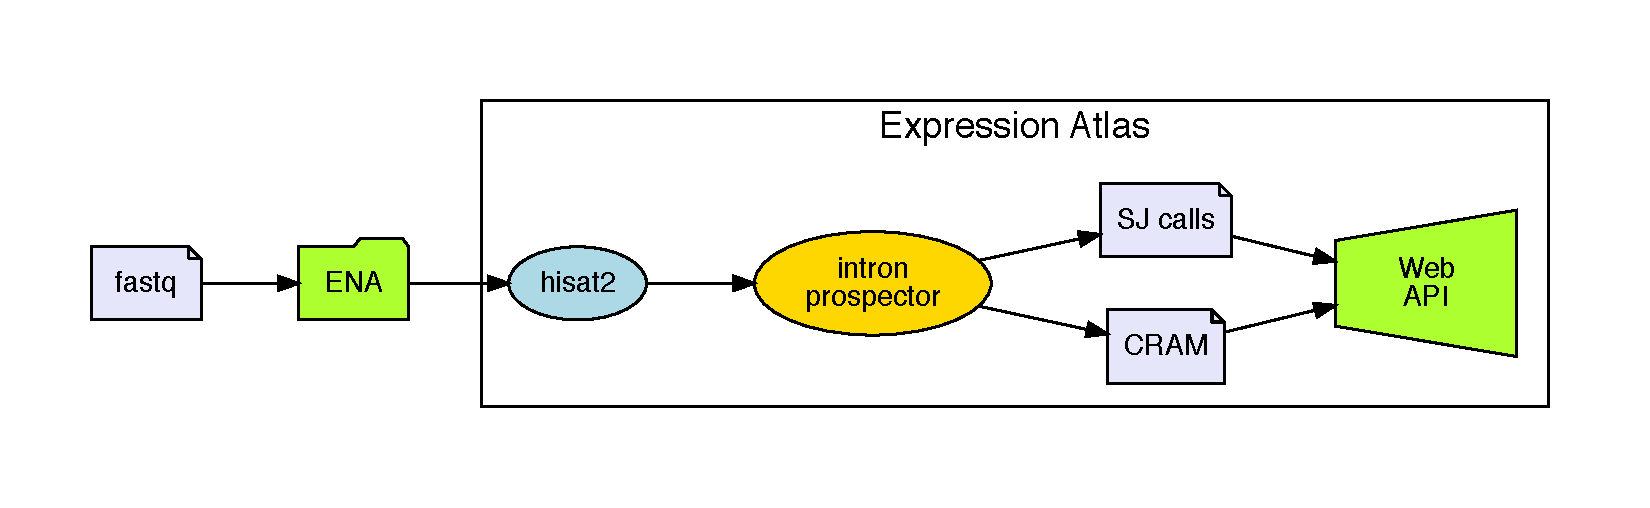
\includegraphics[scale=0.42]{images/calling_at_expression_atlas.pdf}
  \end{center}
\end{frame}

\begin{frame}{Long-read transcript support}
  \begin{itemize}
  \item Supplement and eventually replace GenBank w Iso-Seq \& Oxford Nanopore
    \begin{tightitemize}
    \item Currently a limited number of SRA data sets
    \item CRG \& Brooke's lab
    \item Other sources? 
    \end{tightitemize}
  \item UCSC Nanopore project and Nanopore WGS Consortium
    \begin{tightitemize}
    \item \url{https://github.com/nanopore-wgs-consortium/NA12878/blob/master/RNA.md}
    \item Direct RNA sequencing
    \item $3^\prime$ complete
    \item Also doing cDNA
    \end{tightitemize}
  \end{itemize}
\end{frame}

\begin{frame}{TP53 nanopore direct RNA}
  \vspace{1em}
  \begin{columns}
    \begin{column}{0.5\textwidth}
      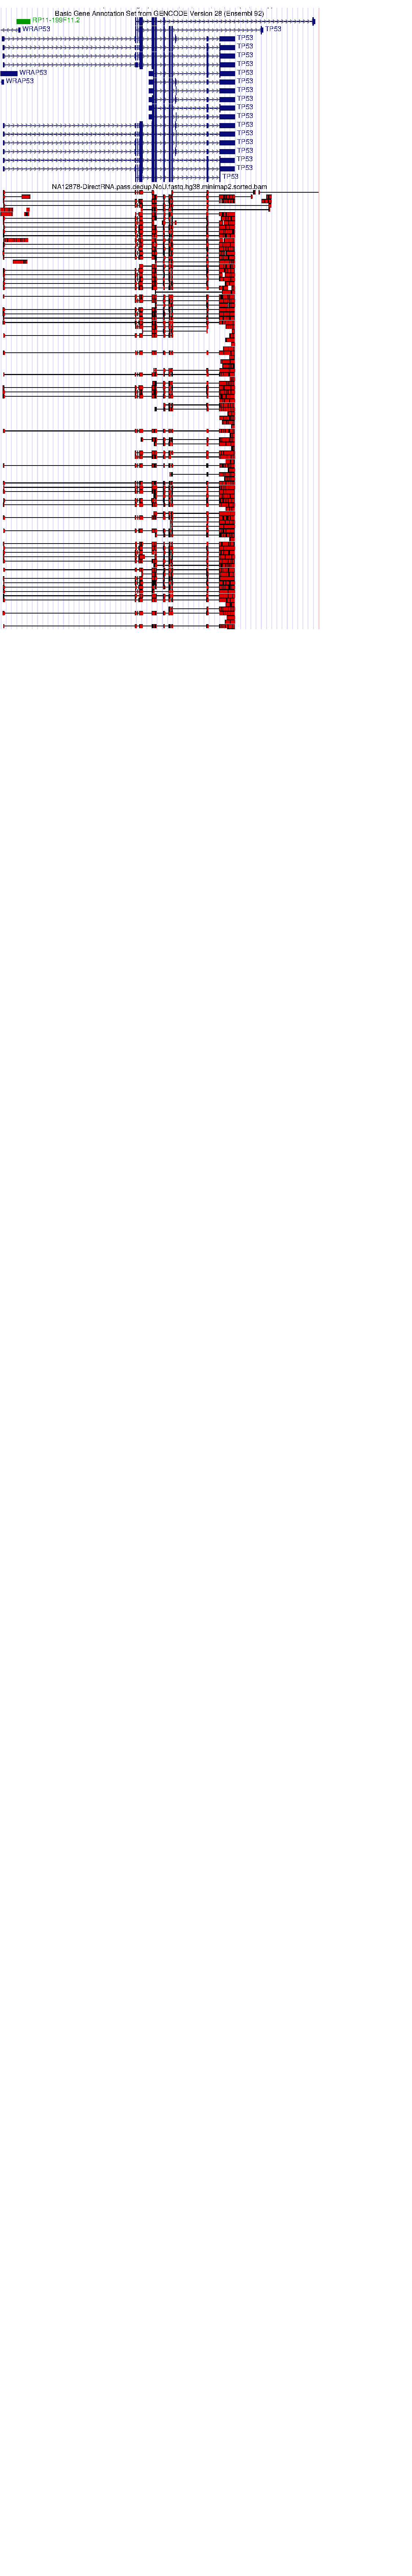
\includegraphics[bb=0pt 0pt 429pt 814pt,clip,clip,scale=0.35]{images/tp53-direct-rna-1.pdf}
    \end{column}
    \begin{column}{0.5\textwidth}
      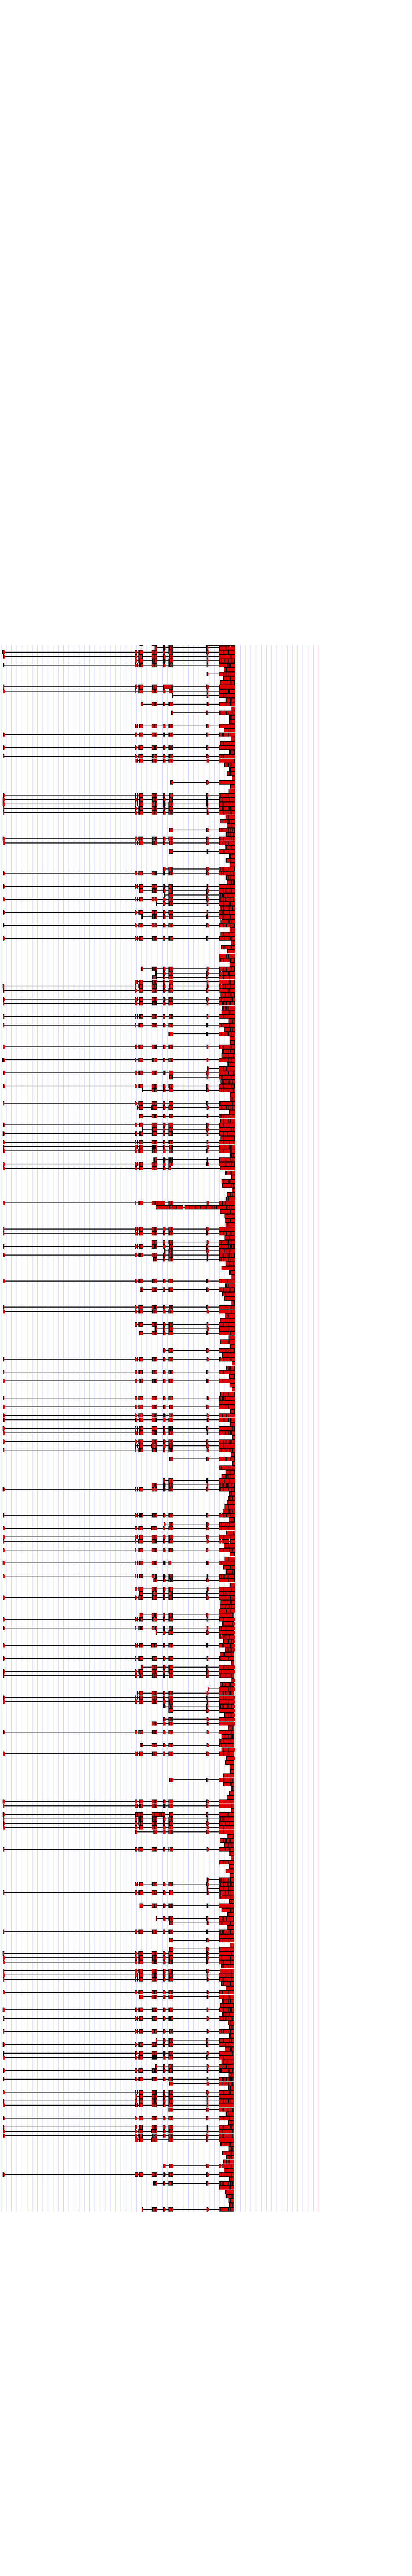
\includegraphics[bb=0pt 0pt 429pt 814pt,clip,scale=0.35]{images/tp53-direct-rna-2.pdf}
    \end{column}
  \end{columns}
'\end{frame}

% -----------------------------------------------------------------------------
\iffalse
\sectionframe{UCSC Browser}
\begin{frame}{}
  \begin{itemize}
  \item 
  \end{itemize}
\end{frame}
\fi

% -----------------------------------------------------------------------------
\begin{frame}{\thetitle}
  \section{Discussion}
  \begin{figure}[b]
    
\includegraphics[scale=0.20]{images/Bugs.jpg}
  \end{figure}
\end{frame}
% -----------------------------------------------------------------------------
\iffalse
\begin{frame}{}
  \begin{center}
    \includegraphics[scale=0.20]{}
  \end{center}
\end{frame}

\begin{frame}{}
  \begin{itemize}
  \item 
  \end{itemize}
\end{frame}
\fi

\iffalse
% nanopore 
\fi
\end{document}
